%!TEX root = ../Master.tex
\chapter{Problem analysis}

In this chapter we will cover different problems associated with indoor navigation in a hospital. We will formulate our initiating problem, based on the issues that we relate to indoor navigation, and navigation in three dimensions. In the problem analysis we will work on the initiating problem, and delimit our initiating problem down to one problem statement, that we will try to solve.

%\{How can indoor navigation in hospitals be optimized by generating a specific route for individuals with different prerequisites?}

\textbf{How can a software solution optimize indoor navigation in Danish hospitals for visitors and patients with different prerequisites?}\label{sub:init}


%!TEX root = ../../Master.tex
\section{Social Relevance}


Technology plays a major role in today's modern society and everywhere you go, you will stumble upon some form of technology. Today's society would not exist without the technological advancements which man has made in the past. Despite this fact, not all technological advancements remain relevant and not all technologies have a use in a modern society. An example of this would be the steam pump. It was once a very important invention and to a degree it still is because it laid the foundation for more advanced technology. However it became obsolete as more advanced technology has made a more advanced pump. Hence the relevancy to society of a certain technology is determined by the use it has, and whether it can compete with existing technologies in its own field.

\subsection{Navigating Today's World}
It can be a daunting task to find your way around today's modern society. Past one's comfort zone the roads may seem infinite and navigating them, an impossible task. This was previously, and still is, alleviated with the use of maps, however maps will not dynamically update your current position and reading a map can be very difficult for the inexperienced. However, in the 1980's, the world saw the advent of GPS \cite{gps_advent}. GPS navigation improved upon navigation via maps as it plans the route for the user, while at the same time dynamically updates the user position, which removed the need for the user to keep track of their position. This made the need for reading a map and planning a route superfluous. These improvements over the traditional map meant that GPS navigation would be capable of competing with the existing technology at the time (i.e. maps, compass etc.). GPS navigation has remained a relevant technology to this day because navigating around the world is just as necessary and challenging now as it has ever been.

\subsection{Navigating indoors}
GPS navigation helped make outdoor navigation easier, but the system does not work indoors, due to limitations with the signal and accuracy \cite{gps_tech}. With facilities getting larger and more complex every day, the need for indoor navigation has never been greater.

While outdoor navigation saw the advent of GPS navigation, indoor navigation has had to rely on old fashioned navigation where the user has to manually position and navigate themselves, as described in \cref{sec:anal_nav}. With the increasing use of GPS navigation, which requires little to no user action, it would seem anything but likely that people have become more skilled at manual navigation. This poses the problem of how people can navigate reliably indoors.

What makes this a problem is the fact, that if individuals cannot get to where they need to be, they cannot perform the task they set out to do. This leads to frustration for those involved, be it the visitor at a hospital or the patient awaiting a visit. While navigation may seem simple to many it is imperative to acknowledge that it becomes easier with knowledge of the area and newcomers most definitely will struggle to find their way.

Many solutions to this have been proposed and developed over time, however it remains evident that none of the solutions have managed to solve the problem to satisfaction, as proved by the continued attempts to solve the problem \cite{skejby_attempt}.

\subsection{Relevance of Better Indoor Navigation}
In recent years the Danish government has restructured and made several cutbacks to the national healthcare system in attempts to save money \cite{cutback_danNHS}, however it was done on the premise that it would not compromise on the quality of the health care provided. This means that the Danish hospitals now have to provide the same level of care for a fraction of the cost and so efficiency improvement has been a key point in the aforementioned restructuring. One of the ways the Danish hospitals have had to deal with the cutbacks is by laying off employees \cite{cutback_firing}\cite{cutback_danNHS}, this means the remaining staff (nurses etc.) have to do more in the same amount of time, so the effective use of the staff's time is crucial.

A 2004 study \cite{timewaste}\cite{timewaste_report}, researching the role of the physical environment in modern hospitals, found that in a 300-bed hospital, the staff spent around 4500 hours per year helping patients and visitors find their way around the hospital. This amounts to around 20 hours a day of time wasted, time that could potentially be saved by better indoor navigation.

With so much focus on effectiveness and saving money, this is an issue that must be considered relevant, and should a proposed solution be able to track positions dynamically it would be able to save even more time as the study also shows that a large amount of time is wasted by the staff looking for medications, patients etc.

\subsection{Summary}
The solution to this problem may not be simple as many complexities arise when dealing with different prerequisites and goals, however it is not a problem that should be overlooked as the potential gains are substantial and amount to both money and time saved and it should save many frustrations for the people as a whole.

%!TEX root = ../../Master.tex
\section{Existing systems} % (fold)
\label{sec:existing_systems}


\paragraph{Phone}
Visitors are able to call the hospital's main number, and ask questions to a live operator. This can be done from any phone but there is no guarantee that a live operator is available.

\paragraph{Signs}
There are signs placed that mark different areas of the hospital. "Main entrance" and "Ambulance entrance" signs can be used to mark key places that the visitor can navigate from\cite{art_Osborne}.
Interior signs are also places in the hospital. These painted to the walls, affixed to doors or windows and others hanging from the ceiling. These describe what room or hall the visitor is in. Some of these signs also contain information about where the different areas of the hospital can be located, often marked by a line of text followed up by a arrow pointing in a specified direction. If the hospital is made up by multiple buildings, they can be numbered in order to navigate people to specific buildings.

\paragraph{Maps}
Maps offers a top-down view of the hospital with all the different locations marked by text or colour\cite{art_Osborne}. The map can be painted on a wall or found in a compact version meant to be carried around. The stationary maps often have a red dot that marks where the reader is. By knowing the current position, the visitor should be able to navigate with more ease as they won't have to look for something recognizable. If the building has multiple floors, the map will be split up into sections in order to cover all the rooms.

\paragraph{The receptionist}
The receptionist can answer questions from the visitors. Very much like the phone, but with some key differences. The phone is more accessible as the one calling does not need to be at the hospital. The receptions has an advantage of being more precise. There will be less confusion as body language can be used in the answering of the question.

\paragraph{Colour coding}
Coloured stripes across the wall or floor that leads to the different areas of the hospital. In the entrance hall the visitors will see a wall with some lines of text with a coloured stripe behind it. One line might say "recovery" and if followed, will lead to the recovery department. Some departments also have an entire theme in a certain colour. In this way, it might become easier for some people to navigate the next time they visit, if they can remember the colours representing the department. 

\paragraph{Porter}
The porter helps patients and visitors get around at the hospital. The porter helps visitors find available beds if they have to stay at the hospital overnight \cite{ugd_port}. 

% section existing_systems (end)

%!TEX root = ../../Master.tex
\section{Individual Stakeholders of Indoor Navigation in Hospitals} % (fold)
\label{sec:interusers}

\sinote{Vi skal afgrænse os fra staff.}

To understand the need for an indoor navigation system, we need to understand the different potential users groups and their needs for an optimized system. In the following segment we will try to bring forth the different motivations for wanting a more optimised and personalized navigation system.

When it comes to indoor navigation in a hospital, there are three main groups we consider individual stakeholders, namely visitors, patients and staff. These groups all have different traits, that might be unique for a single group. However the groups we consider, will only account for the traits acquired while navigating, and not the personal traits of the navigator. So before we describe the differences of our three main groups, we must acknowledge that there are personal traits that might be shared across all of the groups.

Humans have natural differences in their ability to navigate. Some individuals can always tell which way is north, some might lose their sense of direction if they spin in place, and many have a hard time telling left from right, without any visual aid. There are also certain groups of individual who are more prone to having difficulties navigating, such as the elderly, disabled individual or individual affected by mind altering substances. These groups of individual also share a high frequency of visiting hospitals, and so it is increasingly important to address their needs for navigational guidance.

What follows is a closer look at the different needs and traits of the three main groups.

\subsection{Vistors} % (fold)
 \label{par:vistors}
 

An important trait that all types of visitors can share due to the nature of a hospital, is an elevated level of emotional distress. This is often due to the grief or otherwise sadness towards the illness of whom they are visiting. It can also be caused by other things, such as nosocomephobia (the fear of hospitals) which many individual have a variating degree of. These traits can all be impairing, if one requires a focused mind when navigating, and it is important \chnote{source?} to take this into consideration when designing a navigation system. There are two types of visitors that we would like to focus on here, that being those who frequent hospitals and those who do not.

Visitors who do not frequent hospitals, and thus will not have any prior knowledge of the standard infrastructure, will have a hard time navigating the hospital. These visitors will often not be used to navigate any large building, and therefore stationary maps or other guidelines that entails a multitude of actions, which requires memorization, can be hard to adapt to. They will usually prefer asking members of the staff, or using the more simplified yet inefficient forms of navigation, such as counting room numbers or being guided by a friend through a telephone. They will often need confirmation on their current whereabouts and the next course of action.

Visitors who do frequent hospitals, might still share some of the troubles of the non-frequent visitors, but they will however often know, in which quarters the patient they are visiting is situated, and how to get there. But unlike most visitors who do not frequent the hospital, these do not always prepare their visit in full detail, since they might be visiting multiple times a week or even daily. An example of this, could be a parent of a hospitalized child, who decided to drop in during their lunch break. However it just so happened to be, that a part of a doctor's schedule was freed up, and now the child is in another ward, receiving treatment an hour prior to the original schedule. Suddenly, a short visit turns into something much more, because the parent does not necessarily know the details of the rescheduling. Having a loved one confined in a hospital is already an immense emotional stress factor, but also having to deal with navigating to shifting whereabouts, can easily cause unnecessary agitation, which will likely be directed towards the doctors and nurses.

These are suboptimal conditions for a facility working with something as important as human lives, and staff should not be required to handle the stress of visitors, who are having trouble navigating.

%\subsection{Medical Staff} % (fold)

%Just as with the visitors, Medical staff can be divided into two groups, those who frequent the hospital and those who do not. The members of the medical staff who frequent the hospital, will know their way around, at least they will know the part that they are working in, but even then, there can occur navigation problems. 
%\fixme{[Kasper: kan ikke finde nogen kilde der omtaler 'medical staff's problemer med navigation. Hvis det her skal med, skal vi lave et interview. Alternativt kan vi også bare ligge vores fokus hos dem som er hårdest ramt (patienter)n]}

%The other group could contain surgeons with rare specialties, who are only brought in on special occasions, and therefore does not have the layout of the hospital memorized.

\subsection{Patients} % (fold)

Patients who either live at the hospital for extended periods or patients who visit the hospital on a weekly or even daily basis, are considered frequent patients.Emergency patients or patients with a non-recurring medical issue, will be considered non-frequent patients. The latter of the two groups, share a significant amount of traits with the normal visitors, but there are some traits that are more common for patients.

A lot of patients are, by the nature of being a patients, not completely well. Many patients will not have their ability to navigate impaired by their medical condition, but for other it can be greatly reduced, sometimes to the point of non-existence. This could include anything from physical injuries such as broken bones or other conditions that confines a patients his beds, or it could be cognitive disabilities either chronic or temporarily medicinally induced. Other disabilities such as visual impairment and dyslexia \chnote{note?} will often render a visually based guidance system, such as maps, signs and arrows, to be of no virtual help.


\subsection{Summary}

\sinote{Skriv hvilke brugere vi vil have fokus på. Afgræns f.eks. blinde}
\kanote{Her skal der stå en kort tekst der opsumerer afsnittet}
%Solving the problem with indoor navigation will require a possibility to adapt to a multitude of different needs, both when generating a route and when relaying the information to the user. Traditional methods of navigating, such as finding the shortest distance or the fastest path, might not be the best way to generate the route, since special needs of certain users can cause these methods to be counterproductive.


% section Interessents - Users (end)

\sifatal{mangler carstens del}

%!TEX root = ../../Master.tex

\section{Technology} \label{tech}

% \kanote{Der efterfølgende stykke har jeg ikke skrevet. Jeg synes godt vi kan beholde meningen, og så bare skrive det om, så vi indlejrer definitionerne, og ikke referer til andre steder? OGSÅ: ideen om at kort beskrive aspekterne af navigation er godt, men skal det stå her?}
% In order to navigate individuals indoor, it is important to always find the most optimal route based on the users prerequisites. This makes wayfinding technologies very important to our project, and we will cover this in \cref{sub:way}. For any wayfinding technique two parameters is required: a start and an end location. The start location can be determined by positioning the individual. This is done using the methods described in \cref{sub:pos}. Positioning have some requirements that the infrastructure has to comply with, we will define those requirements in \cref{sub:infra}.

Before anyone can develop an optimal solution to a problem, it is necessary to understand the technology at one's disposal. But since understanding technology is time consuming, it is important to analyse which to focus on. In the following section, we have selected the technologies that we estimated have the most relevance to our problem, and analysed how they might be used in a possible software solution. It is important to note, that we have only analysed technologies, that support a possible solution to the entirety of our problem, with a few exception. These exceptions have been included because their hold a prominent role in a common optimal solution to a similar problems.

The analysis of the technologies follows a certain simple method. We describe the different existing digital technology, and analyse their relevance to our initiating problem. We then outline the function of a given technology, and determine its relevance by examining why the technology is in use, and specifically which traits makes the technology relevant for our problem. We subsequently describe any undesirable traits which will decrease the usefulness in a possible solution.

\subsection{Method} \label{sub:techmethod}
This method gives a good overview of the usefulness of the given technology, without going into much detail. Details, that are deemed important for understanding a solution or is not otherwise easily obtainable, will be included in a later theoretical chapter.




%Teknologier der kan medtages (HVAD & HVORFOR, IKKE HVORDAN): GPS, RFID, QR-kode, Google Maps, Smartphones, Tablets, PDA, Handheld computing/tracking device, accellerometer, WiFi og andre relevante ting.

%!TEX root = ../../Master.tex
\sinote{Afgræns i afgrænsningen; vi vil kun arbejde med software med øje til handheld devices}

\subsection{Handheld Devices} % (fold)
\label{sub:device}

% subsection subsection_name (end)
 	 
Handheld computing/tracking devices, such as smartphones, tablets and PDAs, are all relatively small and users are able to carry them around. Such devices have a screen, with the exception of some older PDAs, and a Wi-Fi or Bluetooth connection module, that allows them to send and/or receive data. This data can then be projected onto the screen, to inform the user.

%The PDA functions as a personal digital assistant, who will keep track of the user's calender or have a calculator program. Two popular PDA's are the iPod touch and BlackBerrie which are still in use. 
%The Smartphone are much alike the PDA, but have other features such as the ability to receive or make phone calls. Smartphones also a varity of apps that allows 3rd party programs to be installed. Such programs could be digital games or social media programs like Facebook or Twitter. Two popular smartphone series would be the iPhoneor the Samsung galaxy.
%The Tablet is bigger in size compared to the PDA and smartphone, and won't fir in the users pocket. They serve almost the same purpose as the smartphones but have more computing power and memory storage. The tablets are used to satisf the needs that laptop covers that a smartphone will not do competent enough. Such needs could be to surf the world wide net, which many do on their laptop or home PC. This can be done on a smartphone but the screen is often seen as too small. The tablet have a bigger screen and thereofre provides a better experience. Two popular tablet would be the iPad and the Surface. 
Devices like smartphones and tablets are already in use, and they are very popular. This means that for many users, a solution with a downloadable program or application, would be easily adapted. Other navigation programs/applications that they have already used, could have similarities with the solution used in this project, which will ease apdaption even more. These devices are also very portable and can be taken to the hospital without much effort. They can also be used to render a map or otherwise assist the user with navigation, for instance through text, sound or pictures.

For these devices to be used as intended, they requires some prior basic digital knowledge. In order to use the device to navigate trough a given method, the user would have to start the device and navigate to the appropriate application in order to get started. This could potentially hinder some users as this could be confusing to them.

One of the caveats of handheld devices is the limited battery capacity. The battery time of a device depends on many factors including screen-on time, processor usage, radio modems etc. As an example a widely used handheld device has a rated \enquote{internet use} battery time of up to 10 hours. \cite{Apple}

When designing the navigation system the limited battery capacity of these handheld devices must be taken into account.
%The modern devices are also fairly expensive which could make them less attractive to users.

%!TEX root = ../../Master.tex
\subsection{Google Maps}
Google Maps is a web mapping service hosted by Google inc. The application is used by some of Google's other products such as Google Transit\cite{Goo_transist}. 

When a user is using on the Google maps application, all information will be downloaded to their device. Information is downloaded when they search on a location or when they drag the map around\cite{Goo_input}. The satellite images are acquired from other companies like Tele Atlas\cite{Goo_Tele} or Zenrin\cite{Goo_Zenrin} and then overlayed with Ground truth\cite{Goo_GT}.
The map will be shown with a top down view like many other maps and will offer satellite images, road maps or dynamic maps. It is also possible to go into Street View which is another Google tool, from where the viewpoint is from the street level\cite{Goo_street}.

Google maps can be used to plan routes, show earthquakes and even lets you swim with turtles\cite{Goo_Turtle}.

Google maps is relevant for this project as they have made it able to show maps inside buildings, as seen at Aalborg Universitet, Cassiopeia\cite{Goo_Indoor}. This system could be implanted at the hospital so it would show the different floors and have them all mapped. Instead of using a GPS, Google Maps Indoor uses Wi-Fi hotspots and telephone towers to locate their target\cite{Goo_Indoor}.

It is not certain that every complex has enough Wi-Fi hotspots or telephone towers nearby. Therefore this may not be a general solution.

%!TEX root = ../../Master.tex
\subsection{Location Fingerprinting}
In location fingerprinting, there are to main tecniques that have been choosen for this project. It is "QR-code" and "RFID".
Location fingerprinting is method of recognizing devices by giving them a electronic fingerprint, such as a unique id.

\paragraph{QR-code} % (fold)
QR-codes are barcodes that returns data when scanned. The code is represented by black boxes on a white square grid background. All by how the boxes are arranged, the code will represent different data.

In order to read the data, a scanner has to be used. A camera from a smartphone can be used for this purpose, as long there are an app that supports this particular format. Such apps can be found on nearly all smartphones\cite{QR_smart}. The QR-code can be used to lead users to websites, and are used often in different kind of commercial ways\cite{QR_url}.

It is easy to read the QR-code if you already have an app installed on your smartphone. It is also easy to make your own codes as Google have released a free tool to generate them\cite{QR_Google}.It is also rather easy to set up a QR-code system in a effective way\cite{QR_easy}.

The relevance for this project is how it will take little to no time to set up\cite{QR_rel1}, and how some people already knows how use them as they are widely spread\cite{QR_spread}. Even if a code is damaged it will still be usable, all up to 30\% of the code can be missing\cite{QR_dama}. This also means it will be possible to implant images in the code and still have it working\cite{QR_image}.

A reason for not to use the codes could be that some users might exploit the system. If they print their own codes with links to certain websites it could be a very unpleasant experience for the other users\cite{QR_urlbad}. In worst case scenarios they could be used to steal personal information\cite{QR_information}.
In order for the codes to be efficient, they also have to placed at many locations at the hospital. The users should always be able to find them when they want to use them. This could leave to frustration if they seems to be nowhere to find for the user.


\paragraph{RFID}
RFID (Radio Frequency Identification) is a radio technology that makes it possible, just like barcodes, to identify different objects. the main difference between these two technologies is that the barcode is a line of sight technology, and RFID is wireless, as long as it is within visible distance. The readable distance varies depending on the type of RFID tag. The information exchanged can be in many different formats such as text, numbers, audio or video. It depends on the size of the RFID tag built-in memory. 

There are, different RFID tags, as they can be passive, active or battery-assisted. Tags can be read-only "one time read" or read-write "multiply times", have a serial number, or can be plank for the owner to write something on it. To put it into perspective to our project, a read-only tag can be used to find an object such as a printer that does not change its name or property. Read-write tag, can be used to track patients, the information can chance the name and CPR number to match the person who wears it.  


%!TEX root = ../../Master.tex
\subsection{Accelerometer}

The Accelerometer is a transducer that measures acceleration. The acceleration could be static if the device is at hold an only affected by gravity, or dynamic if it moves around\cite{acc_engi}. Accelerometers is used in many different ways and are also used in a lot of different applications, such the PlayStation 3 DualShock 3 remote\cite{acc_ps3} or in a Nokia 5500 sport\cite{acc_nokia}.


The accelerometer is able to detect vibrations, change of altitude or direction\cite{acc_engi}. Some accelerometers works by relying on the piezoelectric effect that delivers electronic output from a variety of crystals inside the device\cite{acc_piezo}. This electronic output can then be read by a computer and used to generate information about the state of the accelerometer.


The accelerometer is among other used because it can reliable be applied in car GPS systems. It uses the technique dead reckoning that estimates ones position based on previously coordinates and current vector movement\cite{acc_dead}. The accelerometer has also proven itself useful in some science aspects, such as earthquake investigations or monitoring active volcanoes\cite{acc_vulkan}. 


The accelerometer is relevant for this project, as it can be used to position the users if it is incorporated in a device that is going to be carried along side the current user. In this way it could be used to see if the user is following the generated path or if he/she have moved outside of it. The accelerometers that could be used for this project could be the LIS302DL as it is rather cheap and compact\cite{acc_price,acc_lis302dl}. This accelerometer have already been incorporated in the original iPhone\cite{acc_iPhone}.


A downside with the accelerometer is that it can not stand on its own. The accelerometer is unable to position itself and will therefore need to work alongside another system, such as a GPS or wifi and etcetera. 

\subsubsection{Wi-Fi} \label{wifitech}
Wi-Fi is a technology that uses radio waves to transfer data between electronic devices. Computers and handheld devices make use of Wi-Fi, together with many other electronic devices \cite{wifi_devices}.

Wi-Fi can be used in location fingerprinting using triangulation. This works because every Wi-Fi hotspot has an unique id and a known location. An estimated position of a Wi-Fi receiver can be calculated based on the signal strength to every Wi-Fi hotspot. It is then possible to calculate a position  \cite{Liu2007}.

Wi-Fi can connect to the internet via a wireless access point such as a router. Wi-Fi allows places that normally would not have internet connection, like sheds or gardens, to connect. This is possible as the router or wireless access point will allow the device to get a connection.

This is widely used as they serve as an convenient way of getting internet access. They are fairly easy to set up and used widely in the private homes and also used at a greater scale such as an airport \cite{wifi_works}. It is an convenient way of getting internet access as the user is in no need of getting a cable that physically have to be connected to a router.

It is relevant for this project as there have been invested in installing Wi-Fi hotspots at the Danish hospitals \cite{wifi_hospi}. This means it would be possible to set up a service that will connect trough these hotspots.

A problem with Wi-Fi is how, as by Danish law, the hospital will have to log data from the users who connect to it \cite{wifi_log}. In order to only log the users who are using the Wi-Fi, a password would be optimal as it will prevent people bypassing the complex from automatically connecting. The range is also a limitation as typical routers will support a range of 46 meters indoor \cite{wifi_range}. Walls will reduce the strength of the signal, which means some areas of the complex might no have a good enough connection \cite{wifi_wall}. Handheld devices consumes more power when Wi-Fi is active, and quickly drains the battery as data is send and received \cite{wifi_batt}. The amount of power used is reduces as the device goes into a low power mode, which is activated once it has no more data to send. It goes into hight power mode when it is sending/receiving data and stays there for the duration of which it is sending/receiving the data.


%!TEX root = ../../Master.tex

\subsection{GPS}

Global Positioning System, GPS is a satellite-based positioning system. Satellites emits a signal, a time-stamp and current position. A GPS receiver measures the distance from itself to any satellite, by the time it took to receive the signal at the speed of light. When the positions and distances of multiple of satellites is known, its possible determine the GPS receivers position by trilateration \cite{Dempster2013}. It is possible to use GPS all over the world as long as there a clear line of sight to the satellites. Due to the signals not being able to pass through walls and roofs, means that it is suitable for indoor use \cite{GPS_about}.

 
%%!TEX root = ../../Master.tex


\subsection{Positioning}\label{sub:pos}

  Triangulation is a method used for estimating the position of an object. The method uses the properties of triangles. Triangulation has two derivatives: literation and angulation.

 \subsubsection{Lateration}

  Lateration is commonly used technique for positioning.  Lateration uses the distance between known locations and and the point to be determined, to estimate the location.\cite{tri_lateration}  There are two types of lateration two dimensional and three dimensional. The two dimensional are use in robots that navigates in only one plane, like robot vacuum cleaners. 
  lateration in three dimensions are used in GPS positioning, and other practical applications for positioning.

  \subsubsection{Angulation}

  Angulation uses the technique called Angle of Arrival (AOA), which can compute the location of a source. The parameters needed are as minimum two relative angles between a remote point and the source, and the distance between the remote points. The source is at the location where the lines formed by the angle direction lines intercept. 

  In 2D, as few as two remote points are needed, given the source is not directly in between the remote points. However to improve accuracy and remove ambiguity  another remote point is needed. In 3D, as few as three remote points are needed. However as with 2D, another remote point improves accuracy and removes ambiguity. \cite{Liu2007, Sun2009, Boontrai2009}


  \subsubsection{Location Fingerprinting}


  Location fingerprinting is another techinque used for positioning. It refers to the algorithms that first collect characteristics (fingerprints) of a scene and then matches these a priori characteristics with the characteristics of the location the source is in, to determine the source' location.

  There are two stages for location fingerprinting. The offline state where a site survey is performed in the environment. The characteristics of known locations are stored in databases. In the online state, these a priori characteristics are used to match the location of the source.

  The main challenge of location fingerprinting is the possibility of variating signal strengths corrupting characteristics data.

  \subsubsection{Summary}


  All of the above described technologies need remote points to find a position. As described in \cref{sub:infra}, many hospitals have WiFi hotspots located around the hospital. These WiFi hotspots can be used as the remote points, given that the coverage of the network is good.
%%!TEX root = ../../Master.tex
\section{Leading Technologies}

http://www.wifarer.com/hospitals
http://www.meridianapps.com/products
http://www.smartindoor.com/
https://www.indooratlas.com/


\subsection{Position Technologies}

  \subsection{Satellites}

  \subsection{Cellular Communication Network}

  \subsection{Infra-red}

  \subsection{Blue-tooth}

  \subsection{WIFI}

  \subsection{Summary of Position Technologies}

\subsection{Positioning Techniques}

  \subsection{Cell of Origin}

  \subsection{Angle of Arrival}

  \subsection{Angle difference of Arrival}

  \subsection{Time of Arrival}

  \subsection{Time difference of Arrival}

  \subsection{Triangulation}

  Triangulation is a method used for estimating the position of an object. The method uses the properties of triangles. Triangulation has two derivatives: literation and angulation.

 \paragraph{Lateration}

  Lateration is commonly used technique for positioning.  Lateration uses the distance between known locations and and the point to be determined, to estimate the location.\cite{tri_lateration}  There are two types of lateration two dimensional and three dimensional. The two dimensional are use in robots that navigates in only one plane, like robot vacuum cleaners. 
  lateration in three dimensions are used in GPS positioning, and other practical applications for positioning.
  We will only explain three dimensional lateration.
  \begin{figure}[h!]
  \centering
  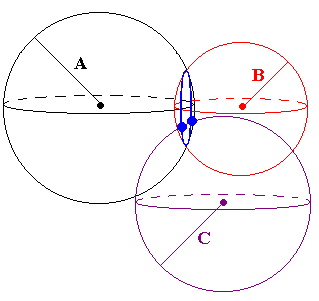
\includegraphics[width=3in]{trilateration}
  \caption{Example of lateration with three know positions.\newline Source: http://ixbtlabs.com/articles/gpssystem/}
  \label{fig:trilateration}
  \end{figure}
  

  Trilateration in three dimensions is possible in fare most situations if and only if the distance to three known positions is defined or possible to calculate.
  If we know a distance to one of these three positions we know that the point we are seeking is in the surface of a sphere, with center at the know position, and with a radius equals to the distance to the center. This is illustrated on figure \ref{fig:trilateration} as the surface of the sphere A.

  The intersection of two spheres is a circle. By determining the distance to a second know point it is possible to circumscribe the range of possible position to a smaller area.
  This is illustrated as the blue circle on figure \ref{fig:trilateration}, and is the intersection between sphere A and B.
  A third sphere that overlaps the intersection between the first two spheres, will mark 2 points where all three spheres is collapsing. In fare most situations there are only one of these locations that lies on the Earth's surface, the other point will often be fare in to the sky or deep inside earth. So by sorting one point from, there is only one possible position left. 
  In some very rare situation it is possible that both point lies on the Earth's surface, and in such situations the use of four spheres will determine witch of the to positions is the right one.



  \paragraph{Angulation}

  Angulation uses the technique called Angle of Arrival (AOA), which can compute the location of a source. The parameters needed are as minimum two relative angles between a remote point and the source, and the distance between the remote points. The source is at the location where the lines formed by the angle direction lines intercept. 

  In 2D, as few as two remote points are needed, given the source is not directly in between the remote points. However to improve accuracy and remove ambiguity, another remote point is needed. In 3D, as few as three remote points are needed. However as with 2D, another remote point improves accuracy and removes ambiguity. \cite{survey_pos, Sun2009, Boontrai2009}

  For example: rangers in location known fire lookout towers can use AOA to pinpoint where the fire is. See \cref{fig:aoa}. A ranger at tower A, sees the fire and notates the bearing to the fire. He then communicates with a ranger at tower B, telling him the general direction of the fire. The ranger at tower B now notates the bearing to the fire from his perspective. The fire can now be pinpointed from the 2 remote points (given the fire started in a 2-D world). The fire is where the 2 angle direction lines intercept. Ranger A at tower C can verify this position by also noting his bearing. \cite{compassdude_triangulation}

  \begin{figure}
    \centering
    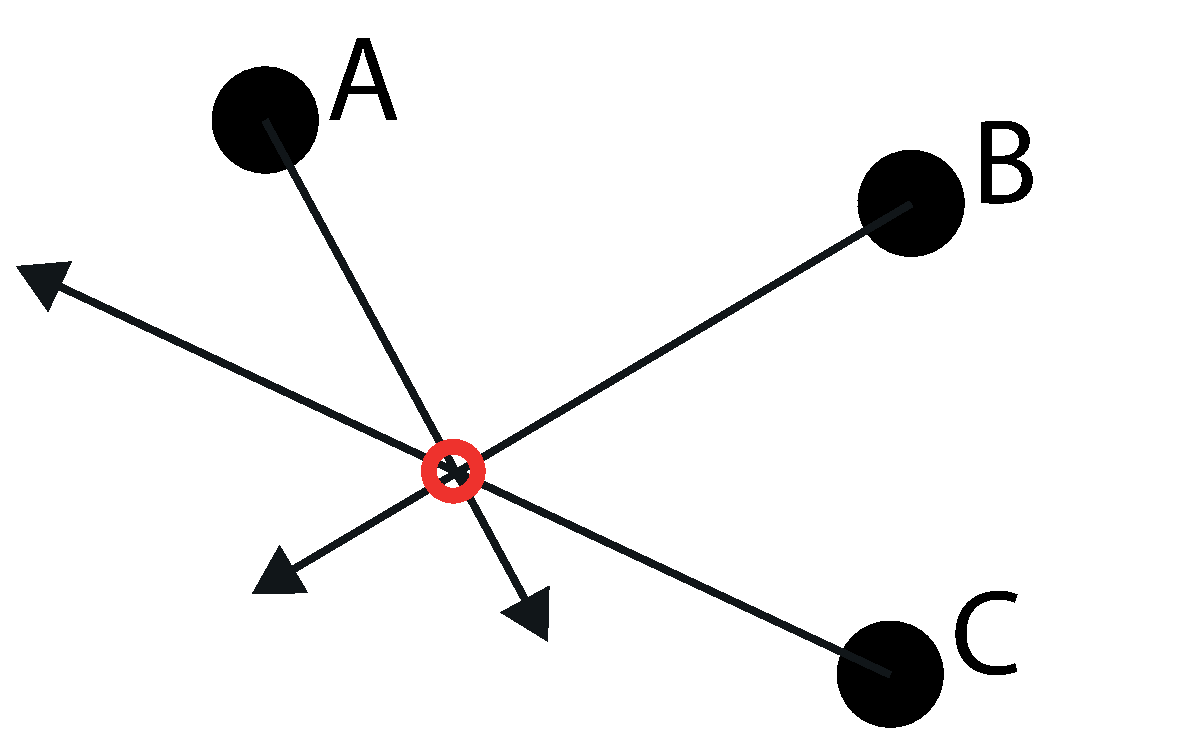
\includegraphics[width=\textwidth]{aoa.eps}
    \caption{Example of fire lookout towers positioning a fire using AOA.}
      \label{fig:aoa}
  \end{figure}

  The advantages of AOA are the few remote points needed in order to estimate a position. Another advantage is the independency of time synchronization.

  The disadvantages of AOA are the need of large and complex hardware requirements, and degradation of the location estimate as the target moves away from the measuring units. In order to perform accurate position of the target, very accurate angle measurements need to be performed. This can become a problem if the measuring is done in wireless networks, because of shadowing, multipath reflections arriving from misleading directions etc. Therefore angulation is best performed in free space.

  \subsection{Location Fingerprinting}

  \subsection{Summary of Position Techniques}

  \subsection{Information Techniques}

  \subsubsection{2 Dimensional map}

  \subsubsection{3 Dimensional map}

  \subsubsection{Text directions}

  \subsubsection{Summary of Information Techniques}

\subsection{Path finding Algorithms}

  Path finding algorithms is used for finding a path between to locations, the source and the destination. By searching its way from the source to the destination, until a path is found. These algorithms also make it possible to calculate the optimal path, I.e. the shortest.

  The algorithms to perform searches they makes use of a weighted graph. A graph, G is a set of nodes V, connected by links E.
  Information about destinations, rooms, entrances and exits would be represented as nodes and hallways and stairs would be represented as links. The distance to travel from node to node via a particular link, would be represented as a weight W(e).

  A important factor of a searching algorithm is correctness and also the time required to calculate the optimized path.
  The algorithms can be rated by their worst-case time, to ensure a responsive performance.


  %\begin{figure}[h!]
  %\caption{A picture of a gull.}
  %\centering
    %\includegraphics[width=0.5\textwidth]{/Images/pathfinding}
  %\end{figure}

  \paragraph{Dijkstra's Algorithm}

  A commonly used algorithm for finding the shortest path is Dijkstra's algorithm. Its loops through steps until all nodes to the target node is optimized with least cost, then points out the shortest path from source node, to target node. The need of every node being evaluated, the complexity of algorithm is proportional with the number of nodes, which means that a lot of computational power is required to calculate the result. The computational cost is calculated O(N*N), where N is the quantity of nodes in the graph.

  Another disadvantage with Dijkstra's algorithm is that its not possible to calculate negative weighted values, which could potentially cause the algorithm to engage in an infinite loop. A negative weighted value could mean saving money over loosing by passing through a certain area.

  We consider the problem: find shortest path from source to target.

  Where P is the source node, Q is the target and R is the evaluating node

  The nodes are subdivided into three sets:

  Set A - Optimized nodes (least costly path from P is known)
  Set B - Temporary nodes (evaluated cost of path from P but not part of set A)
  Set C - Remaining nodes

  The links are subdivided into three other sets:

  Set I - Links used in the set A
  Set II - Not part of set I (one and only one link of this set will lead to each node in set B)
  Set III - Remaining links (rejected or not yet considered)

  At first all nodes is assigned to set C and all links to set III, P is then assigned to set A.
  Then we loop through following steps until Q is part of set A.

  Step 1. Consider all the links r connecting the node just assigned to set A. If R is part of set C assign to set B and assign r to set II.
  If R is part of set B, then investigate if the use of link r is less costly from P to R than the existing link in set II. If less costly assign link r and reject existing link in set II, otherwise reject r to set III.

  Step 2. For each node in set B where there'Ps only one path in set I and set II, the node with minimum cost from P is assign to set A and with the corresponding link assign to set I.

  %\subsubsection{Bellman-Ford Algorithm}
%%%not relevant right now
  %is based on 3 separate algorithms


  \paragraph{A* Algorithm}

  Firstly A* is an informed search algorithm, where Dijkstra's is uninformed. A* utilises the principle of a heuristic estimation to determine which node to test next.

  - If h is zero, then only g affects the result and making it work like Dijkstra's algorithm

  - If h < g, the algorithm will guaranteed find the shortest path from source to target, at a slow running time.

  - If h == g, the algorithm will only extract the best path, but this not always possible due to obstacles.

  - If h > g, the algorithm will find a path fast not its not always the optimal.

  This means that the heuristic estimation should be reasonable, and not overestimate the distance between to the evaluating node and the target node. But should be just right for the final chosen path to be the optimal path and the for the complexity of the algorithm to be at a minimum.

  \paragraph{Summary of Algorithms}

  %SCHEME OF ADVANTAGES AND DISADVANTAGES
  %======================================

